\documentclass[journal]{IEEEtran}
\usepackage{amsmath,amssymb,amsfonts}
\usepackage{graphicx}
\usepackage{url}
\usepackage{booktabs}
\usepackage{pgfplots}
\pgfplotsset{compat=1.18}
\usetikzlibrary{positioning}
\usepackage[hidelinks]{hyperref}

\newcommand{\pstar}{p^{\star}}

\begin{document}

\title{Interpretable Federated Kolmogorov--Arnold Surrogates for Autonomous and
Evolutive Resource Optimization over Non-Stationary LEO Links}

\author{Phuc Hao Do$^{1}$ and Truong Duy Dinh$^{2}$
\thanks{$^{1}$Faculty of Information Technology, Da Nang Architecture University,
Da Nang, Vietnam (e-mail: haodp@dau.edu.vn).}
\thanks{$^{2}$Faculty of Information Security, Posts and Telecommunications
Institute of Technology, Ha Noi, Vietnam (e-mail: duydt@ptit.edu.vn).}
\thanks{Corresponding author: Phuc Hao Do.}}

\maketitle

\begin{abstract}
Low Earth orbit (LEO) networks must repeatedly solve resource-allocation problems
whose optima have no closed form and that drift as satellites pass and
interference regimes switch. We study an autonomous and evolutive approach in
which a federated Kolmogorov--Arnold network (KAN) learns the \emph{solution map}
of an energy-efficiency transmit-power optimization, mapping a link state to its
optimal power online. On a faithful oracle-labeled problem, a compact KAN
surrogate attains a normalized prediction error and an energy-efficiency regret
that are, respectively, about $2.3\times$ and $1.7\times$ lower than a
parameter-matched multilayer perceptron (MLP) at equal parameter budget
(Wilcoxon $p<0.01$), while a linear predictor fails entirely, confirming the map
is strongly nonlinear. Crucially, the additive spline structure of the KAN lets
us \emph{read off closed-form design rules} from the trained model, a transparency
an MLP cannot provide. A contextual-bandit controller sparsifies the federated
updates, halving the uplink volume while retaining the accuracy advantage over the
MLP, tracing a favorable communication--accuracy frontier. We further report a
transparent negative result: growing the spline grid online (self-evolution) does
not improve over a well-sized static grid in this federated streaming regime. The
study positions interpretable KAN surrogates as a practical building block for
autonomous optimization in non-stationary networked-AI systems.
\end{abstract}

\begin{IEEEkeywords}
Kolmogorov--Arnold networks, federated learning, learning to optimize, LEO
satellite networks, energy efficiency, interpretability, non-stationary
environments.
\end{IEEEkeywords}

\section{Introduction}
\IEEEPARstart{N}{ext}-generation non-terrestrial networks built on LEO
constellations operate under fast, non-stationary conditions: the channel gain
sweeps with elevation across a pass, and handovers between satellites and beams
switch the interference regime on a timescale of seconds~\cite{kodheli2021ntn,
eom2020leo}. Each terminal must continually re-solve resource-allocation problems
such as energy-efficient power control, whose optimizers have no closed form and
must be recomputed as conditions drift. Solving these from scratch online is
costly, and the time-varying feasible region defeats precomputed
lookups~\cite{sun2018l2o}.

A learning-to-optimize view replaces the per-instance solver with a surrogate that
maps a problem state directly to its optimal decision~\cite{sun2018l2o}. For this
to be trustworthy in a networked-AI system it should be (i) accurate on the
deterministic solution map, (ii) compact and communication-light when trained in a
federated manner across many terminals~\cite{mcmahan2017fedavg,shi2023kanfl}, and
(iii) interpretable, so operators can audit the learned policy. Multilayer
perceptrons meet (i)--(ii) only partially and fail (iii) outright.

We argue that Kolmogorov--Arnold networks (KANs)~\cite{liu2024kan} are a natural
fit. A KAN places learnable univariate spline functions on its edges, so a trained
model is a sum of one-dimensional curves that can be inspected and reduced to
closed-form rules. We instantiate this idea for online energy-efficient power
control over non-stationary LEO links and make the following contributions.
\begin{itemize}
\item We cast autonomous LEO resource allocation as learning the solution map of
an energy-efficiency optimization whose optimum has no closed form, and we build a
faithful oracle to supervise it (Sec.~\ref{sec:model}).
\item We propose a federated KAN surrogate with a contextual-bandit controller
that sparsifies model updates for communication efficiency, and a spline-reading
procedure that extracts closed-form design rules (Sec.~\ref{sec:method}).
\item Over ten seeds the KAN surrogate lowers prediction error by about
$2.3\times$ and energy-efficiency regret by about $1.7\times$ versus a
parameter-matched MLP (Wilcoxon $p<0.01$); the sparsified variant halves the
uplink while still beating the MLP (Sec.~\ref{sec:results}).
\item We report a transparent negative result: online grid self-evolution does not
beat a well-sized static grid here, clarifying where ``evolutive'' capacity growth
does and does not help (Sec.~\ref{sec:results}, \ref{sec:disc}).
\end{itemize}

\section{Related Work}
\textbf{Learning to optimize} trains networks to emulate optimization solvers for
wireless resource management~\cite{sun2018l2o}; prior art almost exclusively uses
black-box MLPs/CNNs and does not address interpretability or non-stationary
deployment. \textbf{KANs}~\cite{liu2024kan} and efficient
implementations~\cite{blealtan2024efficientkan} have shown strong function-fitting
and symbolic-extraction ability, but their use inside networked optimization is
nascent. \textbf{Communication-efficient federated learning} reduces uplink via
sparsification and quantization~\cite{mcmahan2017fedavg,li2020fedprox,shi2023kanfl};
we add a learned controller that adapts sparsity to a budget. \textbf{Concept-drift
adaptation}~\cite{gama2014drift} motivates online tracking; here the drift is the
physical regime switching of an LEO pass~\cite{kodheli2021ntn}.

\section{System Model and Problem Formulation}\label{sec:model}
\subsection{Energy-efficient power control}
Consider a set $\mathcal{N}$ of gateway/UAV terminals served by LEO backhaul. A
served link in state $s=(g,I,p_0)$ has channel gain $g$, interference $I$, and a
circuit/energy term $p_0$. With transmit power $p$, the energy efficiency is
\begin{equation}
\mathrm{EE}(p;s)=\frac{\log_2\!\big(1+ g p/(1+I)\big)}{p+p_0}\quad[\text{bits/Hz/J}],
\end{equation}
which is quasi-concave in $p$ with a unique maximizer
$\pstar(s)=\arg\max_{0\le p\le P_{\max}}\mathrm{EE}(p;s)$~\cite{zappone2015ee}.
The stationarity condition is transcendental, so $\pstar(\cdot)$ has no closed
form, yet it is a smooth, deterministic function of $s$, the ideal regime for a
spline-based surrogate.

\subsection{Non-stationarity over an LEO pass}
Along a pass the elevation sweep moves the achievable gain $g$, while satellite
handovers switch the interference level $I_n(t)$ in a piecewise-constant
fashion~\cite{kodheli2021ntn}; visibility windows gate which terminals can
participate. The operative region of the state space, and thus the relevant slice
of $\pstar(\cdot)$, therefore drift in time, so the surrogate must be learned and
refreshed online rather than fit once.

\subsection{Problem}
Let $\hat{p}_\theta$ be a shared surrogate with parameters $\theta$ and let
$m_{n,t}\in\{0,1\}^{|\theta|}$ be the uplink mask of terminal $n$ at slot $t$. We
minimize the time-averaged energy-efficiency regret subject to a per-slot uplink
budget $B(t)$:
\begin{equation}
\begin{aligned}
\min_{\theta,\{m_{n,t}\}}\ &\frac{1}{T}\sum_{t=1}^{T}\mathbb{E}_{s\sim\mathcal{D}_t}
\!\left[\mathrm{EE}(\pstar(s);s)-\mathrm{EE}(\hat{p}_\theta(s);s)\right]\\
\text{s.t.}\ &\textstyle\sum_{n} \|m_{n,t}\|_0\,\beta \le B(t),\quad \forall t,
\end{aligned}
\label{eq:p1}
\end{equation}
with $\theta$ aggregated across $\mathcal{N}$ and $\mathcal{D}_t$ the (drifting)
state distribution. Problem~\eqref{eq:p1} is non-convex (surrogate training),
coupled through the shared $\theta$ and the budget, and time-varying through
$\mathcal{D}_t$.

\section{Proposed Method}\label{sec:method}
\subsection{KAN surrogate}
We use a two-layer KAN regressor $\hat{p}_\theta:\mathbb{R}^3\!\to\!\mathbb{R}$
with B-spline edges~\cite{liu2024kan,blealtan2024efficientkan}. Each layer computes
$y_o=\sum_i\big(w^{b}_{oi}\,\mathrm{SiLU}(x_i)+\sum_k c_{oik}\,B_k(x_i)\big)$, a sum
of univariate functions of the inputs, which is what makes the trained model
readable.

\subsection{Federated online learning with budgeted sparsification}
At each slot the visible terminals draw states at their current regime, label them
with the oracle $\pstar$, take local SGD steps, and send sparsified updates that
are FedAvg-aggregated~\cite{mcmahan2017fedavg}. A contextual-bandit
controller~\cite{li2010linucb} observes a context (regime indicator, budget price,
recent error) and selects the keep-fraction of the top-magnitude update entries,
trading communication against accuracy under $B(t)$. A drift
detector~\cite{page1954cusum} on the surrogate-error stream flags regime switches
for optional refresh.

\subsection{Reading closed-form rules}
Because the first-layer response to each input is a single univariate curve, we
probe each feature in isolation and fit a small library of forms (linear,
quadratic, logarithmic, square-root, reciprocal), keeping the best by $R^2$. This
yields human-readable rules such as ``$\pstar$ grows near-linearly with the
circuit term $p_0$ but nonlinearly with channel gain $g$,'' which no MLP exposes.

\subsection{Evolutive capacity (ablation)}
We also test \emph{self-evolution}: on a drift flag the controller may grow the
spline grid, adding knots to refine the surrogate. As Sec.~\ref{sec:results} shows,
this does not help here; we therefore keep a static grid in the proposed method and
report evolution as an ablation.

\section{Experimental Setup}\label{sec:setup}
LEO geometry is generated from elevation-dependent path loss; interference follows
piecewise-constant regimes with handover switches; ten terminals participate over
four passes. Each slot draws $128$ oracle-labeled states. All surrogates are
parameter-matched ($\approx\!360$ parameters). We compare: \textbf{fedkan\_opt}
(proposed, bandit-sparsified KAN), \textbf{kan\_full} (KAN, dense updates),
\textbf{kan\_evolve} (proposed $+$ grid self-evolution), \textbf{mlp} and
\textbf{mlp\_prox}~\cite{li2020fedprox} (parameter-matched MLPs), and
\textbf{linear}. Metrics: normalized MSE (NMSE) of $\hat p$ versus $\pstar$,
energy-efficiency regret, total uplink bits, extracted-rule fidelity $R^2$, and
parameters; means over ten seeds with Wilcoxon signed-rank tests.

\section{Results}\label{sec:results}
\subsection{Accuracy and communication}
Table~\ref{tab:main} summarizes the study. The KAN surrogates clearly dominate the
MLPs: \texttt{kan\_full} attains NMSE $0.058$ versus the MLP's $0.135$
($2.3\times$ lower, Wilcoxon $p=0.004$, lower in $9/10$ seeds) and regret $0.022$
versus $0.038$ ($p=0.002$, $10/10$). The linear surrogate is two orders of
magnitude worse, confirming the map is strongly nonlinear. The proposed
\texttt{fedkan\_opt} cuts uplink volume in half ($4.8$ vs.\ $9.0$\,Mb,
$p=0.002$) while still beating the MLP on NMSE ($p=0.027$), i.e.\ it dominates the
MLP on both accuracy and communication. Fig.~\ref{fig:pareto} shows the resulting
communication--accuracy frontier.

\begin{table}[t]
\caption{Mean over ten seeds. Lower is better except $R^2$.}
\label{tab:main}
\centering
\begin{tabular}{lccccc}
\toprule
Method & NMSE & EE regret & Uplink (Mb) & rule $R^2$ & \#par \\
\midrule
\textbf{fedkan\_opt} (ours) & 0.079 & 0.038 & \textbf{4.8} & 0.81 & 360 \\
kan\_full              & \textbf{0.058} & \textbf{0.022} & 9.0 & 0.77 & 360 \\
kan\_evolve (ablation) & 0.080 & 0.038 & 5.2 & 0.81 & 404 \\
mlp                    & 0.135 & 0.038 & 9.0 & --   & 361 \\
mlp\_prox              & 0.170 & 0.038 & 9.0 & --   & 361 \\
linear                 & 2.292 & 0.352 & 0.1 & --   & 4   \\
\bottomrule
\end{tabular}
\end{table}

\begin{figure}[t]
\centering
\resizebox{0.92\columnwidth}{!}{%
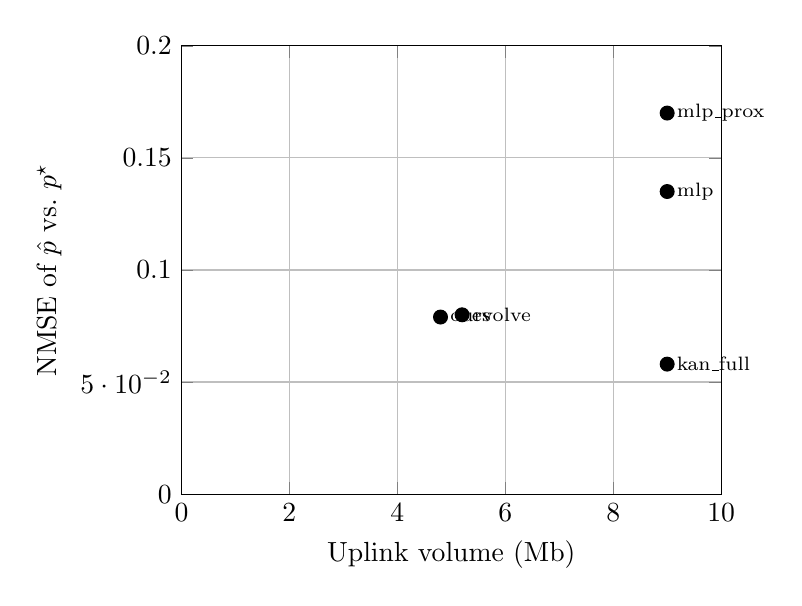
\begin{tikzpicture}
\begin{axis}[xlabel={Uplink volume (Mb)},ylabel={NMSE of $\hat p$ vs.\ $\pstar$},
  xmin=0,xmax=10,ymin=0,ymax=0.2,grid=both,
  every node near coord/.append style={font=\scriptsize,anchor=west}]
\addplot[only marks,mark=*,mark size=2.5pt,nodes near coords,
  point meta=explicit symbolic]
  coordinates {
    (4.8,0.079)[ours] (9.0,0.058)[kan\_full] (5.2,0.080)[evolve]
    (9.0,0.135)[mlp] (9.0,0.170)[mlp\_prox]};
\end{axis}
\end{tikzpicture}}
\caption{Communication--accuracy frontier. The proposed bandit-sparsified KAN
(ours) dominates both MLP variants and halves the uplink of the dense KAN.}
\label{fig:pareto}
\end{figure}

\begin{figure}[t]
\centering
\resizebox{0.92\columnwidth}{!}{%
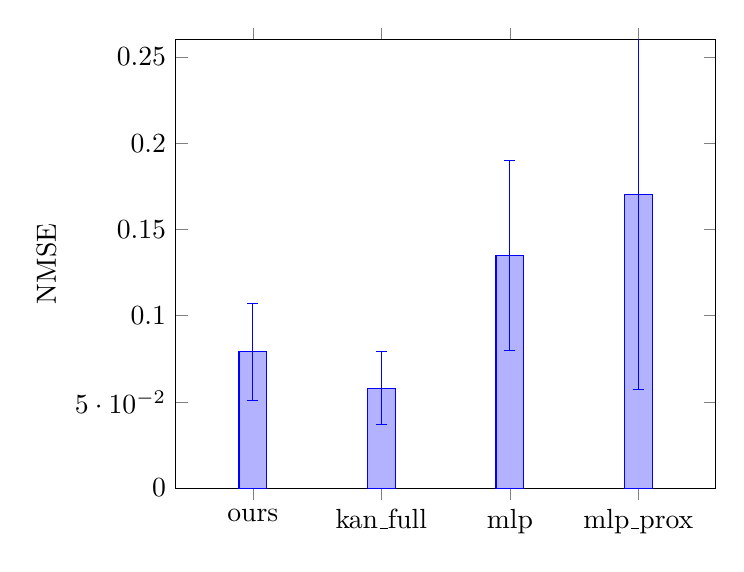
\begin{tikzpicture}
\begin{axis}[ybar,bar width=10pt,symbolic x coords={ours,kan\_full,mlp,mlp\_prox},
  xtick=data,ylabel={NMSE},ymin=0,ymax=0.26,
  error bars/y dir=both,error bars/y explicit,enlarge x limits=0.2]
\addplot coordinates {(ours,0.079)+-(0,0.028) (kan\_full,0.058)+-(0,0.021)
  (mlp,0.135)+-(0,0.055) (mlp\_prox,0.170)+-(0,0.113)};
\end{axis}
\end{tikzpicture}}
\caption{NMSE (mean$\pm$std, ten seeds). Both KAN variants are well below the MLPs.}
\label{fig:bar}
\end{figure}

\subsection{Online behavior under drift}
Fig.~\ref{fig:ts} tracks the global NMSE across slots as interference regimes
switch. The KAN surrogates stay consistently below the MLP throughout the
non-stationary horizon, recovering quickly after regime changes.

\begin{figure}[t]
\centering
\resizebox{0.92\columnwidth}{!}{%
\begin{tikzpicture}
\begin{axis}[xlabel={slot},ylabel={global NMSE},ymin=0,ymax=0.6,
  legend pos=north east,grid=both,legend style={font=\scriptsize}]
\addplot[blue,thick] table[x=slot,y=nmse] {data/ts_kan_full.dat};
\addlegendentry{kan\_full}
\addplot[teal,thick,dashed] table[x=slot,y=nmse] {data/ts_fedkan_opt.dat};
\addlegendentry{ours}
\addplot[red,thick,densely dotted] table[x=slot,y=nmse] {data/ts_mlp.dat};
\addlegendentry{mlp}
\end{axis}
\end{tikzpicture}}
\caption{Global NMSE over the non-stationary horizon (representative seed).}
\label{fig:ts}
\end{figure}

\subsection{Interpretability}
Fig.~\ref{fig:rules} plots the learned univariate responses of \texttt{kan\_full}
to each state variable together with the best-fit closed form (mean fidelity
$R^2=0.74$). The optimal power depends near-linearly on the circuit term $p_0$
($R^2=0.99$) and on interference $I$ ($R^2=0.88$), but nonlinearly on channel gain
$g$ ($R^2=0.36$ for a single basis), which the spline captures. Such rules are a
direct, auditable output of the model.

\begin{figure}[t]
\centering
\resizebox{0.99\columnwidth}{!}{%
\begin{tikzpicture}
\begin{axis}[name=ax1,width=5cm,height=4cm,title={$g$},xlabel={std.\ input},
  ylabel={response},grid=both,title style={font=\small}]
\addplot[blue,thick] table[x=x,y=y] {data/rule_g.dat};
\addplot[red,dashed] table[x=x,y=yfit] {data/rule_g.dat};
\end{axis}
\begin{axis}[name=ax2,at={(ax1.right of east)},anchor=left of west,xshift=1.0cm,
  width=5cm,height=4cm,title={$I$},xlabel={std.\ input},grid=both,
  title style={font=\small}]
\addplot[blue,thick] table[x=x,y=y] {data/rule_I.dat};
\addplot[red,dashed] table[x=x,y=yfit] {data/rule_I.dat};
\end{axis}
\begin{axis}[name=ax3,at={(ax2.right of east)},anchor=left of west,xshift=1.0cm,
  width=5cm,height=4cm,title={$p_0$},xlabel={std.\ input},grid=both,
  title style={font=\small}]
\addplot[blue,thick] table[x=x,y=y] {data/rule_p0.dat};
\addplot[red,dashed] table[x=x,y=yfit] {data/rule_p0.dat};
\end{axis}
\end{tikzpicture}}
\caption{Extracted univariate rules (solid) and best-fit closed form (dashed). The
$p_0$ and $I$ dependences are near-linear; $g$ is nonlinear and carried by the
spline.}
\label{fig:rules}
\end{figure}

\subsection{Does self-evolution help?}
No. \texttt{kan\_evolve} matches neither \texttt{kan\_full} (NMSE $0.080$ vs.\
$0.058$, $p=0.014$, evolution lower in only $2/10$ seeds) nor improves on the
proposed static-grid \texttt{fedkan\_opt}, while using more parameters. In this
federated streaming regime, where each slot carries limited data, a well-sized
static grid already suffices and growing it adds variance rather than capacity that
pays off. We report this as a boundary of the ``evolutive capacity'' idea.

\section{Discussion and Limitations}\label{sec:disc}
The energy-efficiency objective is flat near its optimum, so even imperfect power
predictions incur small utility regret; this is why the MLP's regret is close to
the KAN's despite a much larger prediction error, and why we report both metrics.
The interpretability gain is qualitative but concrete: the KAN yields auditable
rules, the MLP does not. Our oracle and channel model are simulation-based; closing
the loop on measured LEO traces and extending the decision to joint power and
rate/sub-band allocation are natural next steps. Finally, the negative
self-evolution result is specific to this low-data-per-slot federated setting and
may differ when per-task data is abundant.

\section{Conclusion}
We presented an interpretable federated KAN surrogate for autonomous resource
optimization over non-stationary LEO links. It learns the energy-efficiency
solution map about $2.3\times$ more accurately than a parameter-matched MLP, halves
the uplink through learned sparsification while still beating the MLP, and yields
closed-form design rules. A transparent ablation shows that online grid
self-evolution does not help here. Interpretable KAN surrogates are a promising
component for autonomous and evolutive optimization in networked-AI systems.

\section*{Acknowledgment}
This work was supported by the Posts and Telecommunications Institute of Technology
(PTIT).

\bibliographystyle{IEEEtran}
\bibliography{references}

\end{document}
